\documentclass[11pt, a4paper]{article}
\usepackage[utf8]{inputenc}
\usepackage[left=3cm,right=3cm,top=2.5cm,bottom=2.5cm]{geometry}  
% set 11pt and right=6cm for submission

\usepackage{natbib} % we need this so we can use citation and bib properly
\usepackage{enumitem} % allow you to customize your items (like margins etc.)
\usepackage{xurl} % allow URL breaks at any alphanumerical character
\usepackage{hyperref} % allows you to add hyperlink
\usepackage{amsmath} % allows you to use most mathematical features
\usepackage{float,fancyhdr}
\usepackage{amssymb}
\usepackage{setspace} % allows you to change the line spacing
\usepackage{xcolor}
\usepackage{graphicx} % we need this so we can add figures
\usepackage{booktabs}

\title{Conflict Driven Evolution and Urban Development: \\ Evidence from the Holy Roman Empire\footnote{
I thank Davide Cantoni, Matthias Weigand, and my RA colleagues at the Chair of Economic History for helpful comments and feedback. I thank Matthias Weigand in particular for providing me with his own data and for pointing me towards the paper by \cite{schoenholzer2022}.
}
}
\author{Elias Hadj Ammar}
\date{June 27, 2023}

\begin{document}
\onehalfspacing
\maketitle
\thispagestyle{empty}

\begin{abstract}
How does switching between states affect the long-run development of cities, and why? I study this question in the setting of the Holy Roman Empire, using historical data on construction activity and the territorial history of cities. I specifically test the hypothesis that cities benefitted from ownership changes because competition between states selected for higher-quality government. While I show that cities grow faster in the long run after switching states, I do not find evidence that conflict-driven selection played a role in this.
\end{abstract}

\newpage

\setcounter{page}{1}
\doublespacing


% ######################################################

\section{Introduction}



The European state system was forged in conflict. No other continent at any time experienced more war than Europe in the early modern era (\citealp{voigtlnder2013}, p. 174). Wars bring death and devastation to the societies affected by them, but their effects also manifest on the political map --- they play out in a diverse ecosystem of polities that come and go and change size over time. Borders are redrawn and territory changes hands. One can indeed imagine this as an evolutionary process: states compete for resources and powerful states eventually absorb weaker ones. As a result, traits that increase state power --- the ability to win conflicts against rivals --- get selected for, while unfavourable traits are doomed to disappear \citep{levine2021}.

In this paper I study the role of this process in the economic development of the Holy Roman Empire. In particular, I estimate the effect of state power, the trait that conflict selects for, on urban development. If the effect is positive, then the conflict driven evolution of states may partially explain the eventual ascendancy of Europe: by selecting for military success, Europe's violent history may have accidentally produced fiscal capacity, efficient legal systems, and prospering middle classes.

I build my paper on the theory of conflict driven evolution, outlined above, developed by \cite{levine2013, levine2021, levine2022}. Its main contribution is to explain why hegemonies arose in East Asia while balances of power could prevail in Europe: unlike China, the major powers of continental Europe were frequently preyed upon by strong outsiders --- the Vikings, the Swedes, and the English --- which prevented any one state from growing too strong (\citealp{levine2021}, p. 439). It is worth highlighting how the authors model war between states: you win with state power, and state power is simply free resources, i.e. resources above subsistence. If the most successful states are the ones with the biggest surplus, selection should have made Europe increasingly prosperous.\footnote{The basic idea of Darwinian selection has previously been borrowed by economists - for example \cite{galor2002} do the literal version, where humans are subject to selection and accumulate favourable traits over the course of history. More infamously, \cite{clark2007} employs it in an attempt to explain why the Industrial Revolution took place in Europe, arguing that the rich out-bred the poor and passed favourable traits on to their offspring (in Europe but not elsewhere for some reason.)}

The idea that war and conflict can raise the standard of living dates back to \cite{malthus1798}. He reasoned that "positive checks" on the population (war, disease, famine) lead to higher land-labour ratios and therefore higher levels of income per capita. \cite{voigtlnder2013} build upon this Malthusian mechanism and add an explanation for the incessant wars: taxes on those higher incomes filled the treasuries of the rulers, which increased their demand for war --- a luxury good ---, which in turn kept population low. 

By contrast, my story is not about population dynamics but institutions (although it is compatible with Malthusianism). A longstanding tradition in economics emphasises the role of institutional factors in long-run growth (e.g. \cite{north1970}, \cite{delong1993}, \cite{ajr2001}). From this vast literature one theme is especially relevant here: the institution of fiscal capacity, or the state's ability to collect taxes. \cite{tilly1985} argues that the main reason for states to collect taxes is to be able to wage war. In other words, fiscal capacity and state power are tightly linked --- so if conflict selects for state power, then it also selects for fiscal capacity. \cite{gennaioli2015} and \cite{cantoni2023} show that conflict drove state consolidation. \cite{dincecco2012} show that fiscal capacity had a positive effect on growth.

\cite{diamond1997} and \cite{landes1969, landes2006} have argued for the economic benefits of political fragmentation and state competition. \cite{diamond1997} asserts that geography 
remoteness of China deprived it of the benefits of state competition that European states enjoyed throughout their history. \cite{landes2006} makes a similar argument, pointing out how the totalitarianism and bureaucratism that stifled the spread of innovation in medieval China would not have survived long in a more fragmented state system. Fragmentation also plays a central role in \cite{cervellati2022}'s theory.

The closest relative to this paper is \cite{schoenholzer2022} who investigate how switching between states affects the development of cities. They find that switching states affects population negatively in the short run but positively in the long run. Further, they show that this long-run benefit is driven by improved state quality after switching. Similar to the evolution metaphor, they interpret this as "creative destruction": the short run cost of destruction is compensated by the long-run benefit of becoming part of a higher-quality state. However, they do not show explicitly how these improvements in state quality are driven by selection through conflict. They use a dataset with a bigger geographical scope (all of Europe) but lower resolution: they use urban population from \cite{bairoch1988} as a proxy for development, which is only available in intervals of 50 or 100 years. 

The analysis in this paper builds upon that of \cite{schoenholzer2022} and extends it by identifying special cases of switching events: in \textit{conquests} a city is forcefully absorbed into a new state, while in \textit{successions} a city is absorbed into a new state after the rulers of the old state have gone extinct. Comparing the effects of these two types of switches allows me to tease out the effect of state power. Identification is based on the economic assumption that conquests imply state power differentials but successions do not. Specifically, if we consider the universe of all switching events, the average increase in state power from the old to the new owner would be higher for the conquests than for the successions. The reasoning is that conflict --- as in a conquest --- selects the new state for power, but conflict-free successions, depending mainly on dynastic marriages, are more "random". This assumption allows me to use conquests as a stand-in for an increase in state power. Several other assumptions are needed to interpret my results causally.

While I am able to replicate \cite{schoenholzer2022}'s result that switching to another state has a positive effect one century later, I fail to identify a statistically significant effect of state power on urban development. This does not necessarily mean that conflict-driven evolution played no role in the rise of Europe --- several issues limit the statistical power of my test, which might prevent me from finding an effect even if there is one. One of them is that the data I use may not be fully adequate for answering the research question.

The rest of the paper proceeds as follows. Section \ref{sec:background} gives essential historical background information. Section \ref{sec:data} describes the data used in the analysis. Section \ref{sec:empirics} details the empirical approach. Section \ref{sec:results} presents results. Section \ref{sec:discussion} discusses implications and robustness of the results. Section \ref{sec:conclusion} concludes.


% ######################################################

\section{State system of the HRE} \label{sec:background}

The Holy Roman Empire was a powerful monarchy that existed in Central Europe from the Middle Ages until its dissolution in 1806. Though ruled by the Holy Roman Emperor at the Imperial level, it consisted of many small and large territories with their own regional rulers. Before Germany first became a republic in 1918, it is not helpful to think of "states" in the modern sense: while territories may have existed as political entities on paper, they were ruled by aristocrats who handled power in their familial structures \citep[pp. 2-3]{pt2}. These aristocratic families defined the territorial history of the HRE: territories were split by inheritances, joined by marriages and extinctions, and driven to war by struggles for dominance among the noble lineages ruling them. 

When I say "state" in the context of this paper I mean its early modern German equivalent --- the territory of a lineage of rulers, or the lineage itself.


\section{Data} \label{sec:data}

I use data from the \textit{Princes and Townspeople} collection which is based on the \textit{Deutsches Städtebuch} \citep{keyser1939} and \cite{kobler2007}'s \textit{Historisches Lexikon der Deutschen Länder}. Out of the six datasets currently published in the collection, I use those on territorial histories \citep{pt2}, construction activity \citep{pt5} and conflict incidents \citep{pt6} in my analysis.\footnote{I thank Davide Cantoni and Matthias Weigand for giving me access to unpublished yearly versions of the construction and territorial histories data.} I also use the geo-referenced city locations \citep{pt1} to create visualisations. 

From these sources I assemble a panel of cities. City-periods are the unique units of observation. The ultimate dataset contains, in abstract terms, two types of variables: ones that code the \textit{territorial history} of cities, and ones that code the occurrence of certain \textit{events}. Records for each city begin in the 14th century at the earliest and end at the latest with the abolition of the German monarchy in the early 20th century. 

Figure \ref{fig:map_cities_raw} shows the spatial distribution of the 2,390 cities in the original \textit{Princes and Townspeople} data. The reporting boundaries are those of the German Empire in 1937 plus the Free City of Danzig; within those boundaries \cite{keyser1939} claim to list "every settlement that at one point in the history of the Holy Roman Empire was awarded the status of a city" \citep[p. 2]{pt1}.

\paragraph{Territorial histories.} 

A city-by-year panel of territorial history, taken from \cite{pt2}, forms the backbone of my dataset. For each city and each year it identifies the noble lineage to whose territory the city belonged in that year. I use this information to find years in which cities switch from one territory to another. The median city in the original dataset switches territories 5.64 times in its history. 

The original data also records how each city came into the possession of the lineage ruling it. I combine the original 13 types of switches into 3 types: \textit{Conquests}, \textit{successions}, and \textit{other.} I code a switch as a conquest if the original data records it as either "conquest" or "acquisition by conflict", and as a succession if the record says "extinction of lineage" or "inheritance". The remaining categories are classified as \textit{other}.\footnote
{
The other categories are: "no data or regular status", "personal union or marriage", "purchase", "foundation", "secularisation", "decision of the emperor", "gift", "exchange" and "mediatisation".
} 
Cities are ruled by conquering states 16\% of the time, by succeeding states 34\% of the time, and by states that gained possession of them in another way 50\% of the time.

\paragraph{Construction activity.}

The data on construction activity \citep{pt5} and conflict incidents \citep{pt6} both resemble lists of events. The unit of observation is the event, occurring in a specified city at a specified time point. Each entry contains additional information about the type of event and the range of uncertainty for the timing. Because I drop city-period observations with missing construction data from the sample, it is worth briefly outlining how I transform a list of events into a city-period panel of construction activity. First I group and count events that occur in the same city and period. Then I fill the observations in between the events with the value zero. Finally, I code values as missing for periods that are earlier than the first recorded event or later than the last recorded event in a city. I do not set these out-of-range values to zero because I have no way of knowing whether nothing actually happened, or whether the record simply does not cover these periods anymore.

I will regress construction activity on breaks in the territorial history of cities throughout the main part of this paper --- this is not self-explanatory. After all, the research question deals with the effect of switching states on urban economic development. I use construction as a proxy for development because it is available for most cities: out of the 2,390 cities in the \textit{Städtebuch}, 2,177 have at least one construction event linked to them. By contrast, only 207 cities from the \textit{Städtebuch} appear in \cite{bairoch1988}'s dataset of city populations.

The record of construction events is unfortunately not exhaustive and mostly contains notable buildings --- churches, palaces, fortifications, malls, schools, libraries, opera houses, gardens, and the like. It contains residential buildings of some noble families and notable citizens but not of the general population. Even so, there are theoretical justifications for using construction activity as a proxy for growth: If buildings are a normal good, then demand for them should increase with income. While the types of buildings listed do seem to represent state and elite consumption more than general economic activity, the income of these groups is also dependent on the broader economy --- an upturn will increase tax revenues and by extension the disposable income of the state. On a basic level we would expect more new buildings, of any type, in cities that are booming (although the error term is likely large - we might also expect more new buildings in cities that were devastated by war or environmental catastrophes).

In an attempt to understand more about the effects I estimate, I use certain subsets of construction activity as the outcome in alternative specifications. There are 16 types of construction activity in the original data, which I combine into 4 facets: \textit{State construction} consists of palaces, castles, administrative and military buildings. \textit{Private construction} includes malls, economic (banks, factories, restaurants, and more) and private (residential) buildings. Lastly, \textit{construction of public goods} includes infrastructure, social, cultural, and educational buildings, memorials, gardens and parcs.\footnote
{
Churches, monasteries, clerical buildings and town halls are not included in any of the custom subsets of construction activity. They are, however, included in the "All construction" specifications.
}


\paragraph{Conflict incidents.}

I include conflict incidents (sieges, plunders, civil unrest) as a control variable in a robustness check. Conflict in my dataset is simply coded as an indicator whether a conflict incident of any type is recorded in this city and period. I code missing values exactly as I do for construction events.

Note that conflict \textit{incidents} are distinct from conflict as a driver of improvements in institutions. Conflict incidents are events recorded at the city level that often involve the destruction of life or property in that city. The statement "conflict causes weak states to disappear "

\paragraph{Aggregation.}

I aggregate this yearly data into periods of different length. I build yearly, 10-yearly, 50-yearly and 100-yearly versions. I use the 50-yearly version throughout the regressions in the paper. Events are rare enough that this avoids losing too much information to having to drop missing values. Also, some events (conflict as well as construction) are recorded with uncertain timing --- descriptors like "beginning of the 16th century" rather than an exact year. In the aggregated version I include such events if their timing can be assigned with certainty to a 50-year period. The 

The switch indicators are aggregated by summing, to obtain the total number of switches that happen in a period, and the aggregated indicators for construction and conflict take the value 1 if at least one event was recorded during the period. 

\paragraph{Accounting for dropped observations.}

The raw \textit{Territorial Histories} dataset starts out with 1,471,934 yearly observations. I lose two observations per city --- the first and the last year --- while coding switches, for a total of 4,780. I aggregate the remaining 1,467,154 yearly observations into 30,980 observations with 50-year spacing. Of these I drop 16,110 that are not covered by the construction data. Finally, the baseline versions of all specifications in this paper restrict the sample to cities with no more than two lifetime switches. This will remove another 9,975 observations, leaving 6,635 in the baseline sample.

Figure \ref{fig:map_cities_sample} plots the spatial distribution of the cities that make it into the baseline sample. The total number of cities has shrunken visibly compared to Figure \ref{fig:map_cities_raw} --- we can also see, however, that the shrinking appears to have been roughly uniform, preserving the proportions between regions. Only Brandenburg (containing Berlin) and Silesia (containing Breslau) seem to lose disproportionately many observations.

% ######################################################

\section{Regression equations} \label{sec:empirics}

\subsection{Dynamic effects of switching to a new state}

First I attempt to replicate one of the key results of \cite{schoenholzer2022}: that switching states had a positive effect on the growth of cities in the long run. This is an important piece of evidence in support of my hypothesis: states that have successfully taken territory from another are "higher quality", i.e. better for growth. \cite{schoenholzer2022} arrive at this result using an event study with staggered adoption.\footnote
{
    Equation (3), \citealp{schoenholzer2022}, p. 12.
}
The outcome is city population, recorded in intervals of 50 to 100 years. The treatment is switching to another state from one observation to the next. Importantly, a city may change hands multiple times between observations but belong to the same state in the end --- such an event does \textit{not} count as treatment. As the authors show throughout their paper, the short-run effect of switching (either permanently or intermittently) is distinct from the long-run effect of permanently switching to a different state.

I will borrow extensively from this framework. The first regression I run is almost identical to the one described above:

\begin{equation}
\label{eq:sw22}
    construction_{it} = \alpha_i + \delta_t + \mathbf{1}(S_{it} > 0)\beta + 
    \sum_{\tau = -100}^{200} \mathbf{1}(t = e^{NewState}_i + \tau)\pi_\tau + \varepsilon_{it},
\end{equation}

where the outcome $construction_{it}$ is an indicator that equals 1 if any construction activity was observed in city $i$ and period $t$, the variable $S_{it}$ is the number of times a city switched states in period $t$, the variable $e^{NewState}_i$ denotes the first period in which city $i$ belongs to a different state than the previous, and $\alpha_i$ and $\delta_t$ are city and period fixed effects. The coefficients of interest are the dynamic effects $\pi_\tau$ of switching to a new state permanently. 

This is a standard TWFE regression with staggered adoption and dynamic effects. Treatment events are \textit{lasting} switches to another state, i.e. a switching event only counts as treatment if the city belongs to a different state at the beginning of the next period.\footnote
{
    If a city undergoes multiple lasting switches, I create duplicate entries for each different $e^{NewState}_i$. I exclude cities that switch states (permanently or not) more than twice over the sample period. I report results obtained with different exclusion thresholds in Appendix BLANK.
}
This is because I want the coefficients $\pi_\tau$ to capture the effects of the new state's governance, not just of the political and economic turmoil that may be associated with a transition of power. I separately control for other switches by including the term $\mathbf{1}(S_{it} > 0)$ on the right-hand side so that the coefficient $\beta$ absorbs the effect of switching states in the same period.

Since the outcome is binary in this case, we can interpret Equation \eqref{eq:sw22} as a linear probability model: we model $construction_{it}$ as a random variable that follows a Bernoulli distribution with a probability parameter $p$ that is conditional on the right-hand side variables. This way we can interpret the values of coefficients as differences in the probability of construction in a given period. The coefficient $\pi_\tau$ for given $\tau$ is the difference in the probability of construction between two cities $i$ and $j$ with identical time-invariant characteristics, in the same period, who undergo the same kind of switching turmoil in this period. The only difference is that one city underwent a lasting switch to another state $\tau$ periods ago, while the other did not. 

% Since comparisons between cities at different \tau are problematic, we also use the Sun and Abraham estimator (as do SW22).

Based on the theory of conflict-driven evolution we would expect any such difference to stem from the fact that switching states generally means switching to a higher-quality state (due to selection). As such, even though it would be possible in principle to include state fixed effects, it is not a good idea here: state fixed effects would absorb the effect of differences in state quality which we want to capture in $\pi_\tau$ \citep[p. 13]{schoenholzer2022}.

The basic assumption that needs to be satisfied for a causal interpretation of TWFE estimates is parallel trends. This means that, absent treatment, the outcome in cities that received treatment would have followed the same time trend as the outcome in never-treated cities. While it is impossible to empirically prove this assumption (because we cannot observe the counterfactual trend), it is common to check its validity by estimating pre-treatment effects: if the treatment and control group already showed different trends before being treated, there may be an unobserved variable correlated both with receiving treatment and with the outcome, biasing the estimate. For this reason the regression also includes a lead reaching 100 years into the past.


\subsection{Heterogeneous effects of switching}

In the best case, if the identifying assumption is satisfied, the estimates from the previous regression tell us what the effect of switching states is --- however, they cannot tell us why. In the following I attempt to identify the effect of state power, or more accurately, the effect of the difference in selection for state power between conquests and successions. 

Because the \textit{Städtebuch} data compiled by \cite{pt2} records exactly how each city was acquired by the territory holding it, I am able to estimate heterogeneous effects for different types of ownership changes.\footnote
{
Presumably \cite{schoenholzer2022}, having sourced their data on territorial histories from historical maps, lack detailed information about individual switching events. They instead use clever panel decomposition methods (pp. 14-20) and data on state-level characteristics (pp. 21-23) to explain what drives their estimates.
}
For this purpose I extend Equation \eqref{eq:sw22} by interacting the treatment indicator with the type of switching event:
\begin{equation}
\label{eq:baseline}
\begin{split}
    construction_{it} &= \alpha_i + \delta_t + \mathbf{X}_{it} \beta + 
    \mathbf{1}(t \ge e^{NewState}_i) \pi \\
    &+ \mathbf{1}(t \ge e^{NewState}_i) \times
    \mathbf{1}(Conquest_{it}) \cdot \theta_{conquest} \\
    &+ \mathbf{1}(t \ge e^{NewState}_i) \times
    \mathbf{1}(Other_{it}) \cdot \theta_{other} + \varepsilon_{it},
\end{split}
\end{equation}

For clarity I move from the event study to a basic difference-in-differences specification; this way there is only a single coefficient of interest. I simply replace the lead and lag dummies with the post-treatment indicator $\mathbf{1}(t \ge e^{NewState}_i)$. Another minor change is that this equation features a vector of city-year level control variables $\mathbf{X}_{it}$ --- however, in the baseline version of this specification I control only for the dummy $\mathbf{1}(S_{it} > 0)$ that indicates switches in the same period, exactly like in Equation \eqref{eq:sw22}. In a robustness check I will additionally control for conflict incidents.

The more important novelty are the interaction terms: I interact the post-treatment indicator with the type of switch to obtain estimates of how the trends in construction activity differ after different types of switches. I distinguish three categories: $Conquest$, $Succession$, and $Other$. In all cases this refers to how the state currently owning the city came into power --- for example $Conquest_{it} = 1$ means that the state that holds city $i$ at time $t$ acquired city $i$ by conquest. It will be useful to adopt one final bit of notation from \cite{schoenholzer2022} and let $\mathbf{J}(i, t)$ denote the state ruling city $i$ at time $t$.

A key economic assumption is needed, even before the econometric ones, for these interaction terms to tell us anything about state power. It is this: the state power of a city's owner $\mathbf{J}(i, t)$ is correlated with the manner in which the city was acquired by that owner. In particular, I assume that conquests are more strongly positively correlated with state power than successions. Support for this assumption comes from \cite{levine2021}'s model of conflict-driven evolution. BLANK. I will discuss its validity at length later on.

If this assumption holds true, the effect of state power should manifest itself in the difference between the trend of cities acquired by conquest and the trend of cities acquired by succession. Note that successions are the omitted category --- there is no interaction term between the post-treatment indicator and $\mathbf{1}(Succession_{it})$ in Equation \eqref{eq:baseline} --- so that the coefficient $\theta_{conquest}$ captures exactly what we want: the difference in trends after conquests vis-a-vis successions.

The econometric assumption necessary to allow causal interpretation of $\theta_{conquest}$ is a different version of the parallel trends assumption. In particular, it must hold that, had a conquered city i counterfactually been acquired by succession rather than conquest, it would have trended the same as the other cities acquired by succession. BLANK.


% ######################################################

\section{Results} \label{sec:results}

\subsection{Construction activity increases after switching states}

Table \ref{tab:SW22_replication_50y} contains estimates for the coefficients $\pi_\tau$ from Equation \eqref{eq:sw22}. Each column reports the effect of switching states on a different subset of observed construction activity: Column (1) for all types of buildings, Column (2) for administrative, military and representative buildings, Column (3) for private construction, and Column (4) for buildings that provide public goods. The exact definitions of these categories are as described in Section \ref{sec:data}. Note also that a $Period$ is an interval of 50 years that begins with the given year. $Period = -50$ is omitted as the reference category for treated cities. Reassuringly, as the coefficients on $Treat \times Period = -100$ show, there are no significant pre-trends in any of the outcome variables. 

We can see in Column (1) that switching states has no immediate effect on the probability of recorded construction activity. Over the next two centuries, however, the effect grows positive and significant: 100 years after a city switches states, the probability of construction activity is 5 percentage points higher than in cities that did not switch. After 200 years this difference grows to 9 percentage points. These estimates are statistically significant at the 5\% and 1\% level, respectively. Figure \ref{fig:SW_replication} plots the coefficients in Column (1) to visualise these dynamics.

The regression in Column (1) used all construction activity as the outcome, while Columns (2), (3), and (4) use subsets as defined in Section \ref{sec:data}. Almost all the coefficients in the last three columns are insignificant, suggesting that neither of these specific subsets of construction is driving the results. 


\subsection{No evidence for the state power hypothesis}

Table \ref{tab:baseline_50y} shows estimates from Equation \eqref{eq:baseline}. This is a difference-in-differences specification with added interactions to capture heterogeneous treatment effects. As before, different columns use different subsets of construction as the outcome variable. 

I report estimates of the coefficient of interest $\theta_{conquest}$ in the second row. In Column (1) we can see that the probability of construction activity in a given period is 4 percentage points higher following a conquest vis-a-vis after a succession, but the difference is not statistically significant.

The only subset of construction that shows a significant effect is state construction --- palaces, castles, military and administrative buildings. We can see in Column (2) that these are 5 percentage points \textit{less} likely to be built in a city after it was conquered; the effect is significant at the 5\% level. 

The hypothesis was that conflict-driven selection for state power boosts urban growth. Given that my assumption about the difference in selectivity of conquests and successions holds true, the theory would have predicted a positive coefficient $\theta_{conquest}$. The results I obtain instead range from insignificant to negative. They offer no support to the hypothesis.


% ######################################################

\section{Discussion} \label{sec:discussion}

The results in Table \ref{tab:SW22_replication_50y} corroborate part of my hypothesis: switching states within the Holy Roman Empire had a positive effect on the development of cities in the long run. However, the second part of my analysis yields a null result: Table \ref{tab:baseline_50y} shows that the the positive overall effect we saw in Table \ref{tab:SW22_replication_50y} was not driven by conquests. I do not find evidence in support of the hypothesis that selection for state power is responsible for the positive effect of switching.

I test the robustness of this result by estimating some alternative specifications. Table \ref{tab:controls_50y} shows estimates of Equation \eqref{eq:baseline} obtained with different sets of control variables. The outcome is $All \, construction$ in all regressions. Column (1) is identical to Column (1) in Table \ref{tab:baseline_50y} and controls only for switching in the same period. In Column (2) I remove this control. Columns (3) and (4) add conflict as a control variable, once in addition to switching and once without.

Comparing Column (2) to (1), and (4) to (3), we can see that it makes no difference whether we control for switches in the same period or not; the estimates are barely distinguishable. When we control for conflict, however, the coefficient $\theta_{conquest}$ suddenly turns negative, highly significant and large in magnitude. If we trust these regressions, the probability of observing construction in a different year increases by 15 percentage points \textit{less} after conquests relative to successions.

At first glance this may suggest that conflict is an omitted variable in Column (1), biasing the baseline estimate. A closer look at the coefficients on $Conflict$ in Columns (3) and (4) makes this seem unlikely, though: they are very close to zero and not significant by any stretch of the imagination. For conflict to be an omitted variable it would need to be correlated both with the post-$Conquest$ dummy and construction. The first correlation seems plausible --- once-conquered cities may continue to be highly contested, which would imply a positive relationship, or they may enjoy protection from further attacks by their powerful new owner, which would imply a negative relationship --- but the second correlation is zero in my sample.\footnote
{
The coefficients on $Conflict$ in Table \ref{tab:controls_50y} are conditional correlations. Simply computing the correlation coefficient between $Conflict$ and $All\,construction$ yields a value of -0.01.
} The difference cannot be the result of omitted variable bias.

I investigate one alternative explanation: because there are many missing values in the $Conflict$ variable, more than two thirds of observations are dropped between Columns (2) and (3). If the distribution of missing values across observations is not random, the different estimates may be due to starkly different samples. Figure \ref{fig:conflict_map} visualises how including conflict in the regression affects the distribution of the sample across space. The colour of each region codes the share of observations from the baseline sample that remain after dropping observations with missing conflict data. If the spatial composition of the sample stayed exactly the same, the entire map would be a uniform shade. Instead we immediately see big discrepancies: Thuringia and most northern regions all but disappear from the sample, while the more darkly shaded west and south retain between 30\% and 60\% of their observations.

I conduct a number of other robustness checks.

Other things I did:
\begin{itemize}
    \item I limit post-window of the diff-in-diff to 200 years like in the event study; null results
    \item try robust TWFE estimator by Sun and Abraham (2021); null results
    \item use \cite{bairoch1988}'s population data as outcome; null results
    \item regress on data aggregated to 1, 10, and 100 years instead; null results
\end{itemize}


Other explanations for no effect:
\begin{itemize}
    \item states within the HRE may be too similar / competition between them not large enough
    \item successions may also select for state power - maybe you get to enter more advantageous marriages if you are the leader of a powerful state
    \item cities are normally conquered one at a time, while successions usually see many cities switch at the same time - maybe there is a crowding-out of the positive effect, e.g. because the ruler likes one of his newly acquired cities most and neglects the others
    \item the data is just not that well suited to the task; within-R2 is super low in Table \ref{tab:baseline_50y}
    \item had I found an effect, it would have been difficult to show that 

\end{itemize}



% ######################################################

\section{Conclusion} \label{sec:conclusion}

\newpage
\onehalfspacing
\bibliographystyle{chicago}
\bibliography{references.bib}

\newpage
\section*{Tables and figures}



\subsection*{Figures}

\begin{figure}[ht]
    \centering
    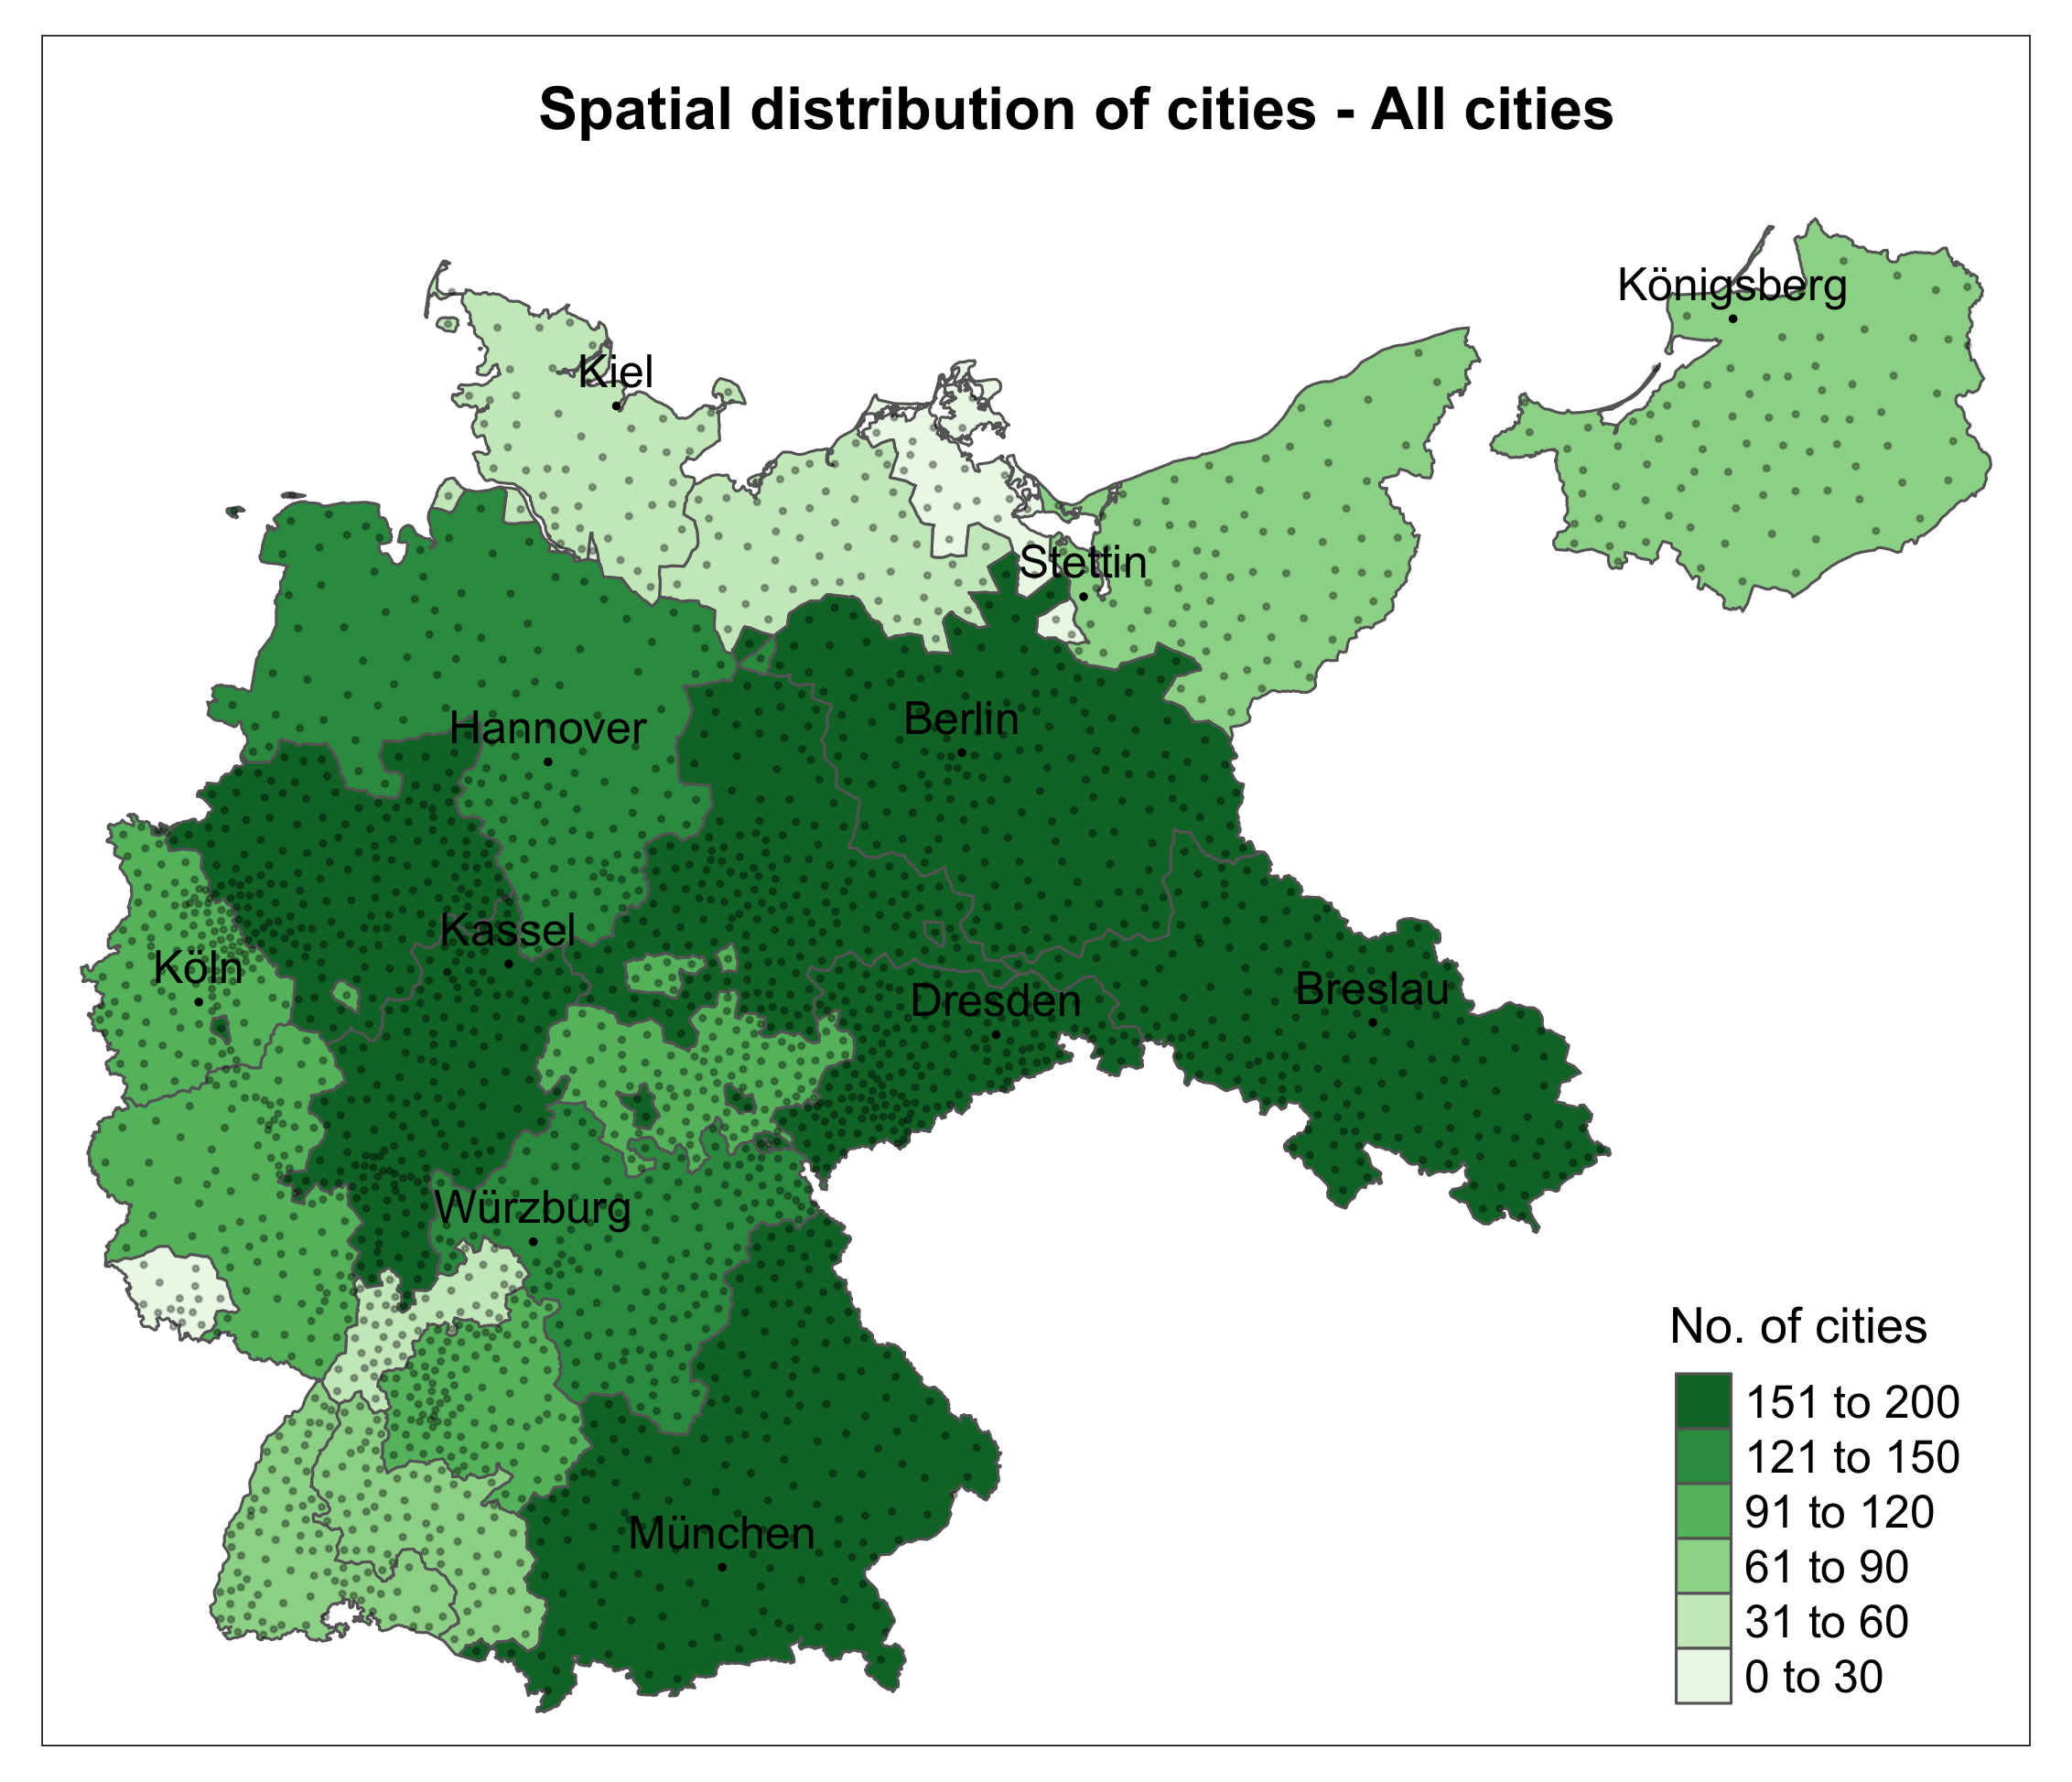
\includegraphics[scale=0.15]{paper/output/descriptive/map_cities_raw.png}
    \caption{Distribution of cities in the \textit{Territorial Histories} dataset \citep{pt2}. Each dot represents a city. Some major cities are identified with labels. Polygons on the map do \textbf{not} represent historical borders; they merely represent regions by which cities are clustered in the \textit{Städtebuch}.}
    \label{fig:map_cities_raw}
\end{figure}


\begin{figure}[ht]
    \centering
    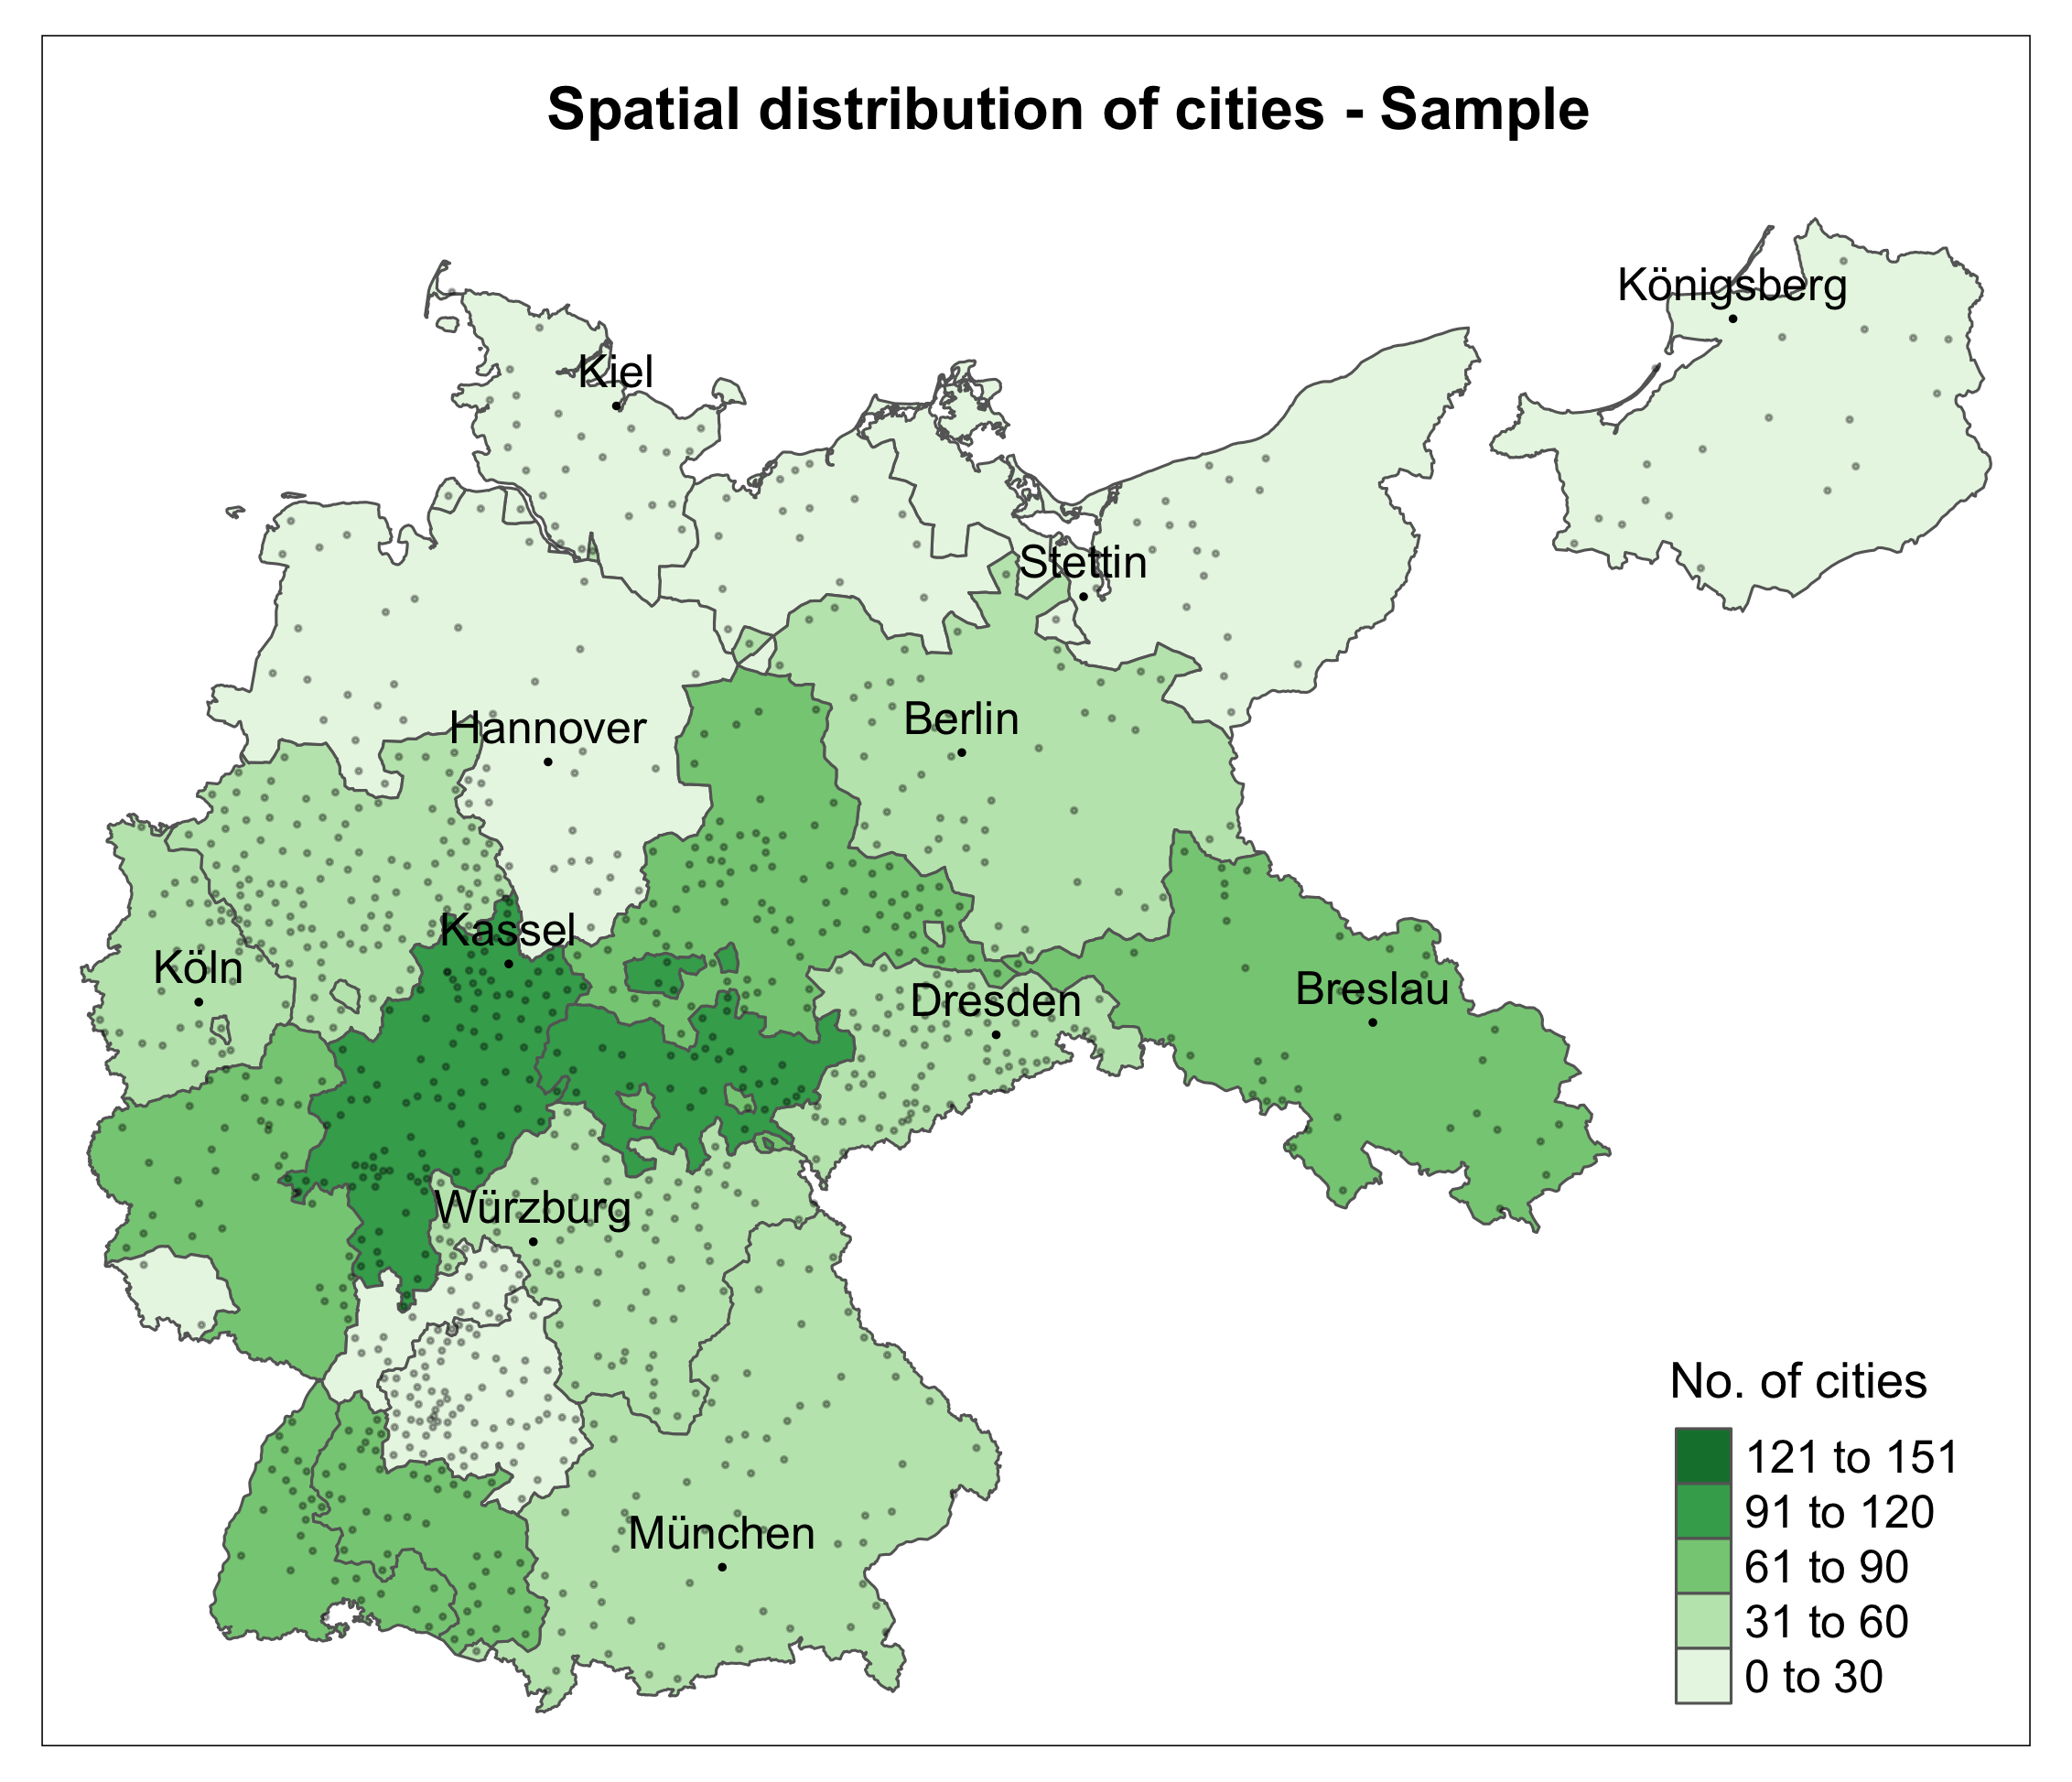
\includegraphics[scale=0.15]{paper/output/descriptive/map_cities_sample.png}
    \caption{Distribution of cities in the baseline sample. Excludes cities that underwent more than two lifetime switches, and cities without any recorded construction activity. Each dot represents a city. Some major cities are identified with labels. Polygons on the map do \textbf{not} represent historical borders; they merely represent regions by which cities are clustered in the \textit{Städtebuch}.}
    \label{fig:map_cities_sample}
\end{figure}



\begin{figure}[ht]
    \centering
    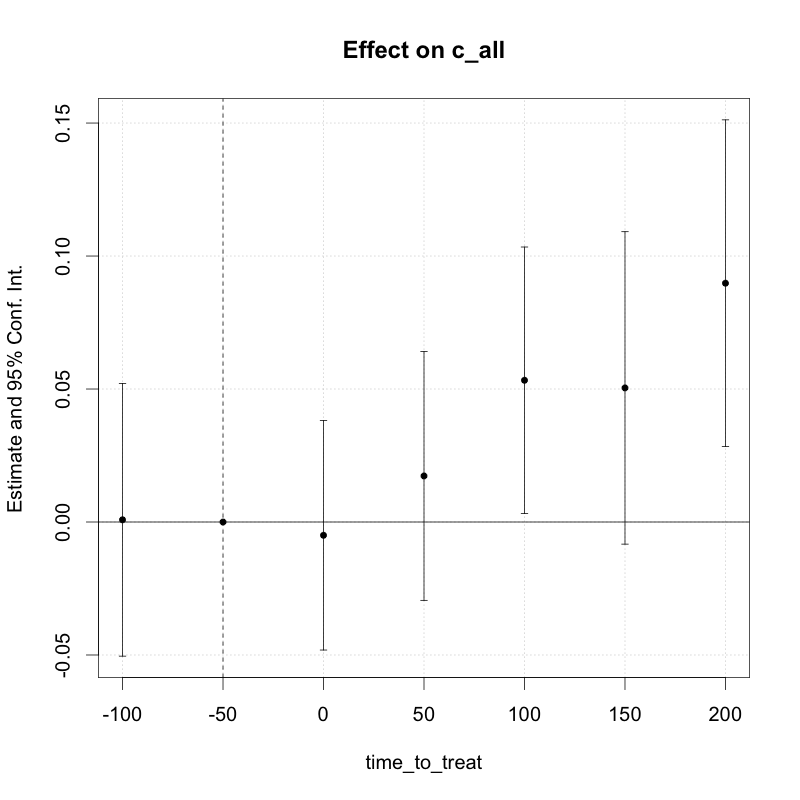
\includegraphics[scale = 0.4]{paper/output/regressions/SW22_replication_50y.png}
    \caption{Dynamic effects of switching to another state. Coefficient estimates from Table \ref{eq:sw22}, Column (1). The outcome variable is the probability that construction activity of any type is observed in the period. The period beginning 50 years before the switch is omitted.}
    \label{fig:SW_replication}
\end{figure}

\begin{figure}[ht]
    \centering
    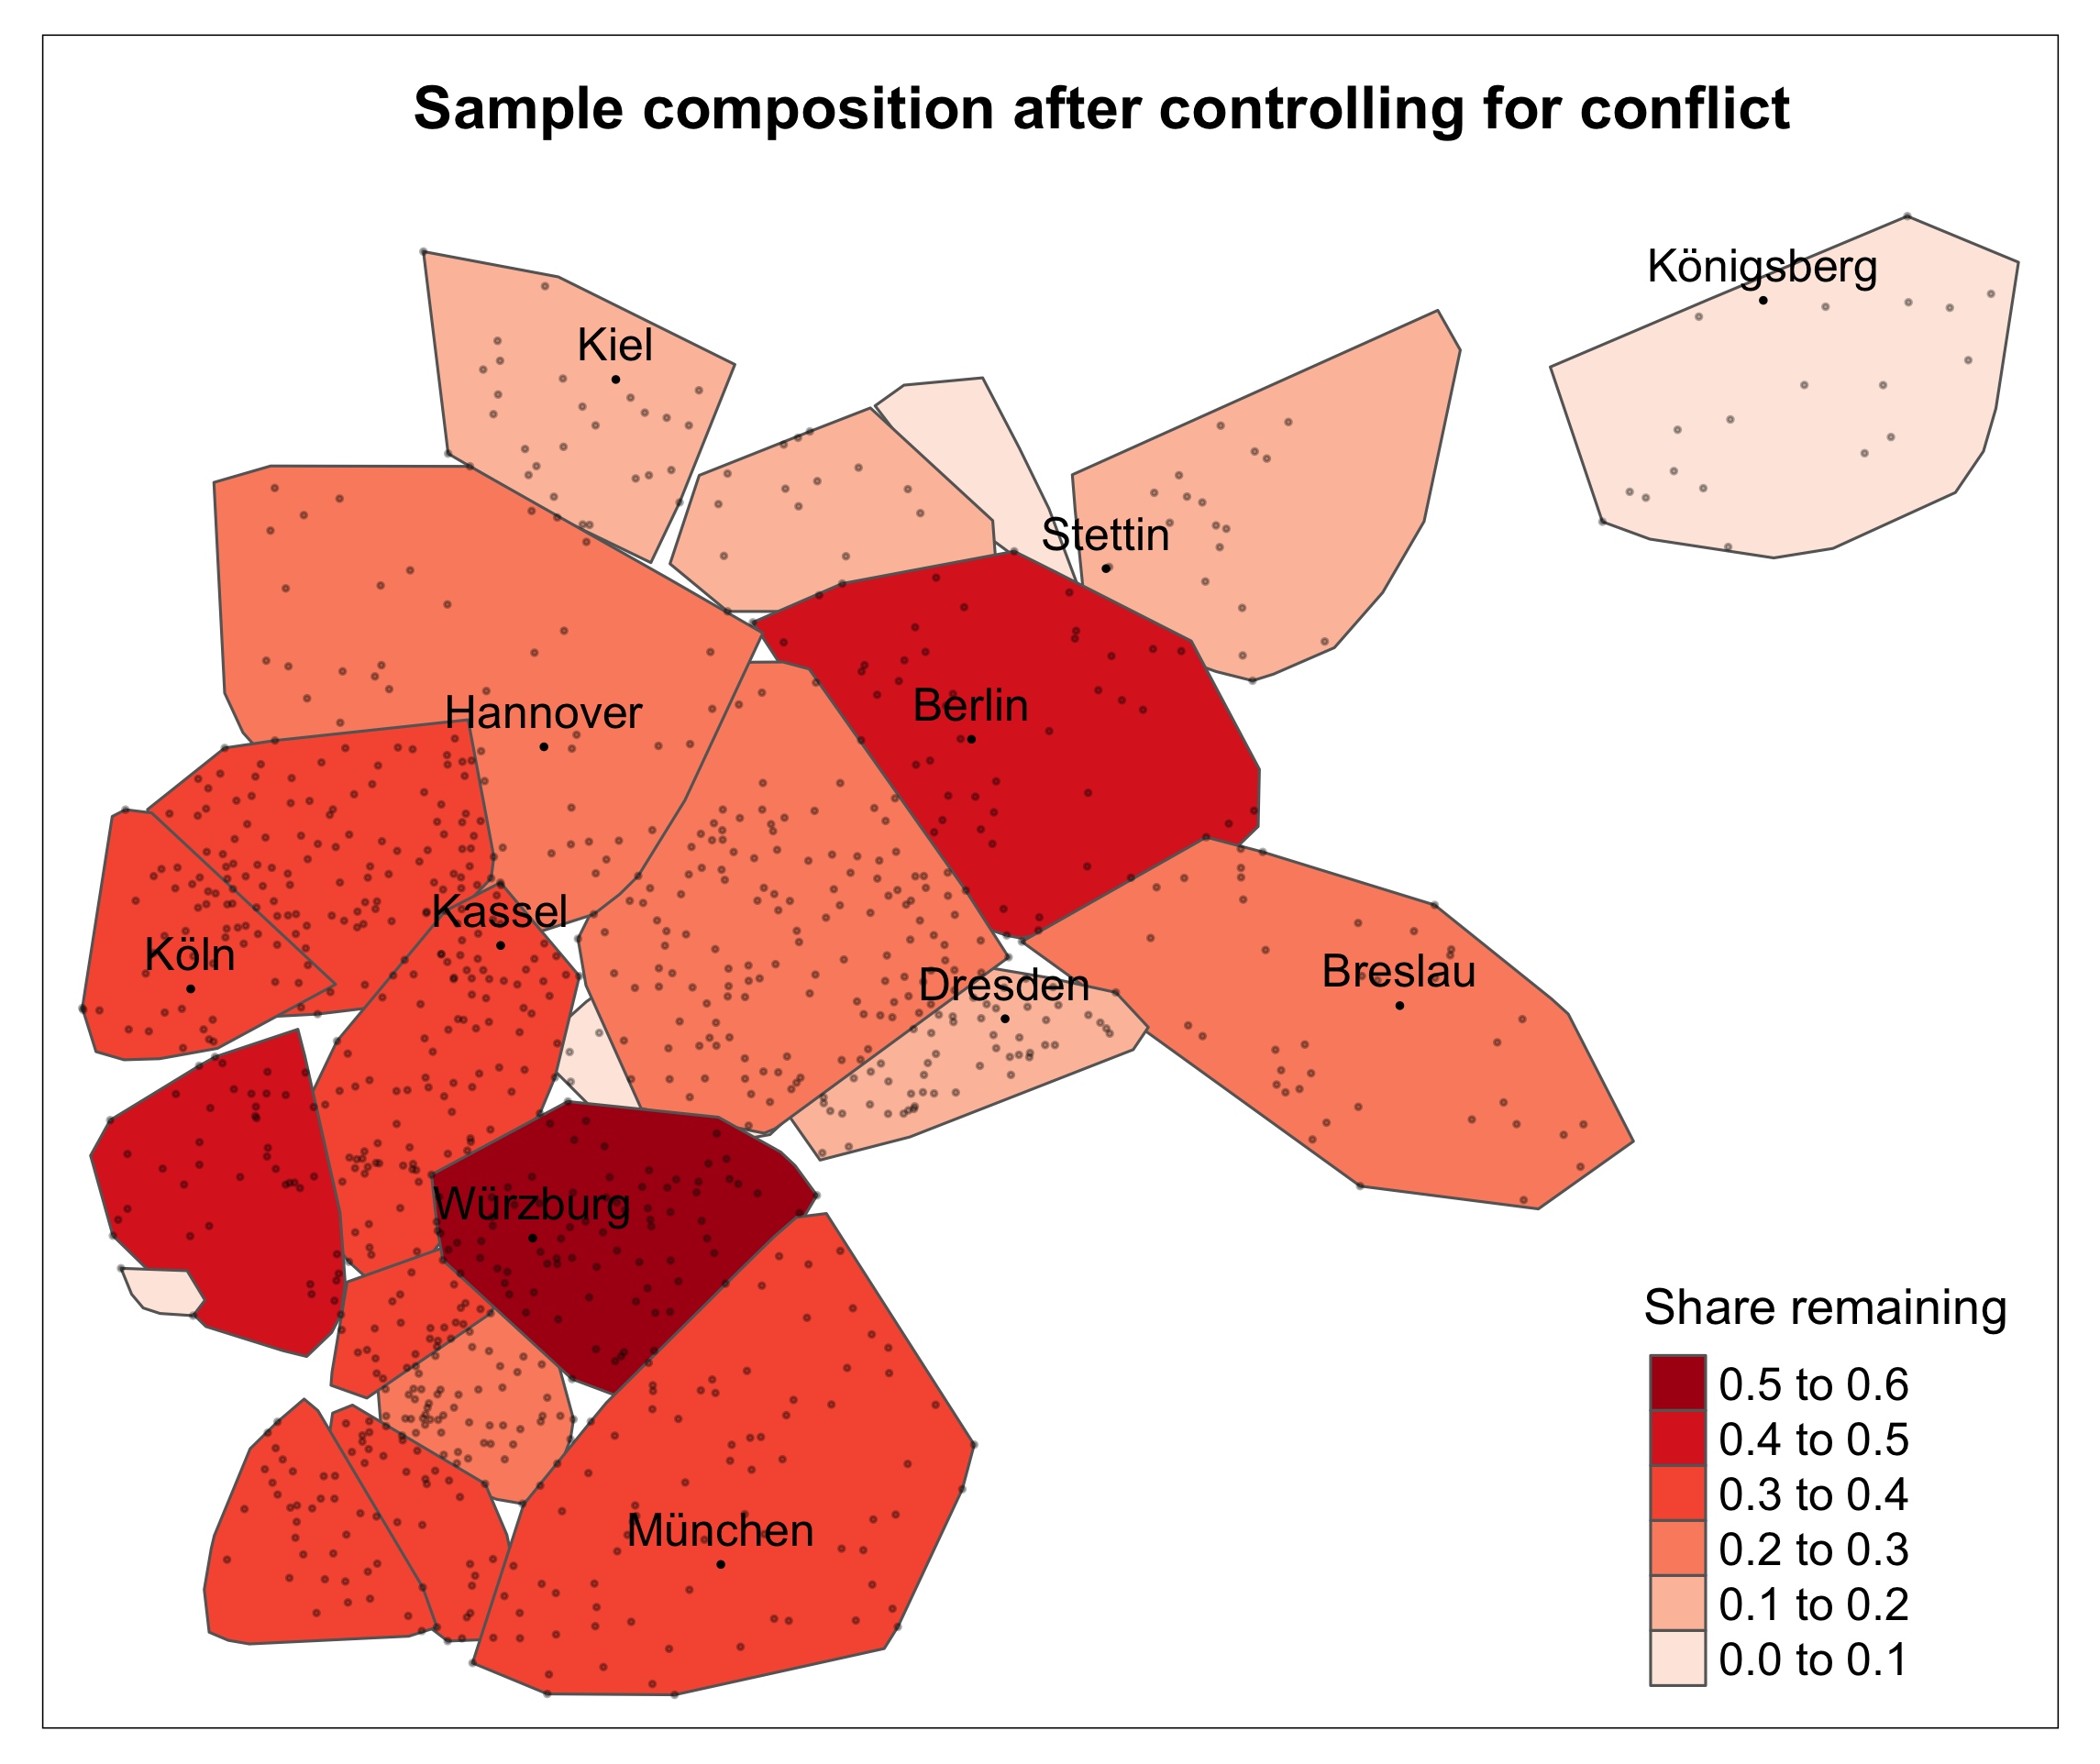
\includegraphics[scale = 0.15]{paper/output/descriptive/map_conflict_NA_50y.png}
    \caption{Share of observations from each \textit{Städtebuch} region with non-missing data on conflict incidents. I code the $Conflict$ variable as missing for a period if it is earlier than the first recorded incident or later than the last recorded incident in a city. Observations with missing conflict data are excluded from the regressions in Columns (3) and (4) of Table \ref{tab:controls_50y}.}
    \label{fig:conflict_map}
\end{figure}

\clearpage
\subsection*{Tables}

\begin{table}[htbp]
   \caption{\label{tab:SW22_replication_50y} Dynamic effects of switching}
   \centering
   \begin{tabular}{lcccc}
      \tabularnewline \midrule \midrule
      Dependent Variables:            & All construction & State  & Private & Public goods\\  
      Model:                          & (1)              & (2)    & (3)     & (4)\\  
      \midrule
      \emph{Variables}\\
      Treat $\times$ Period $=$ -100  & 0.00             & 0.02   & -0.01   & 0.00\\   
                                      & (0.03)           & (0.02) & (0.01)  & (0.02)\\   
      Treat $\times$ Period $=$ 0     & 0.00             & 0.02   & 0.00    & -0.02\\   
                                      & (0.02)           & (0.02) & (0.01)  & (0.01)\\   
      Treat $\times$ Period $=$ 50    & 0.02             & -0.01  & 0.01    & -0.03$^{**}$\\   
                                      & (0.02)           & (0.02) & (0.01)  & (0.01)\\   
      Treat $\times$ Period $=$ 100   & 0.05$^{**}$      & 0.01   & 0.00    & 0.00\\   
                                      & (0.03)           & (0.02) & (0.01)  & (0.02)\\   
      Treat $\times$ Period $=$ 150   & 0.05$^{*}$       & -0.01  & 0.02    & 0.00\\   
                                      & (0.03)           & (0.02) & (0.02)  & (0.02)\\   
      Treat $\times$ Period $=$ 200   & 0.09$^{***}$     & 0.03   & -0.01   & -0.01\\   
                                      & (0.03)           & (0.03) & (0.02)  & (0.02)\\   
      Switching indicator             & -0.01            & 0.01   & -0.01   & 0.00\\   
                                      & (0.02)           & (0.02) & (0.01)  & (0.01)\\   
      \midrule
      \emph{Fixed-effects}\\
      City                            & Yes              & Yes    & Yes     & Yes\\  
      Period                          & Yes              & Yes    & Yes     & Yes\\  
      \midrule
      \emph{Fit statistics}\\
      Observations                    & 6,635            & 6,635  & 6,635   & 6,635\\  
      R$^2$                           & 0.3563           & 0.2799 & 0.3260  & 0.2916\\  
      Within R$^2$                    & 0.0024           & 0.0013 & 0.0007  & 0.0010\\  
      \midrule \midrule
      
      
   \end{tabular}
   
   \par \raggedright 
   Note: Table presents results of estimation equation \eqref{eq:sw22}. Yearly data was aggregated into periods of 50 years. Observations are at the city-period  level. Dependent variables are indicators that take the value 1 if  construction activity of the respective type was recorded. Standard errors are  clustered at the city level. *, **, and *** denote significance on the 10 percent, 5 percent, and 1 percent  level, respectively.
\end{table}


\begin{table}[htbp]
   \caption{Test Title}
   \centering
   \begin{tabular}{lcc}
      \tabularnewline \midrule \midrule
      Dependent Variable: & \multicolumn{2}{c}{Construction}\\
      Model:                                               & (1)           & (2)\\  
      \midrule
      \emph{Variables}\\
      Switching to another state $\times$ Selection $=$ 1  & 0.01 (0.03)   & 0.04 (0.05)\\   
      Switching to another state $\times$ Selection $=$ 3  & 0.04 (0.04)   & -0.15$^{***}$ (0.06)\\   
      Switching to another state                           & 0.02 (0.03)   & -0.010 (0.05)\\   
      Switching indicator                                  & -0.008 (0.03) & -0.09 (0.06)\\   
      Conflict                                             &               & 0.01 (0.03)\\   
      \midrule
      \emph{Fixed-effects}\\
      City                                                 & Yes           & Yes\\  
      Period                                               & Yes           & Yes\\  
      \midrule
      \emph{Fit statistics}\\
      Observations                                         & 6,635         & 1,955\\  
      R$^2$                                                & 0.3553        & 0.4245\\  
      Within R$^2$                                         & 0.0009        & 0.0071\\  
      \midrule \midrule
      \multicolumn{3}{l}{\emph{Clustered (City) standard-errors in parentheses}}\\
      \multicolumn{3}{l}{\emph{Signif. Codes: ***: 0.01, **: 0.05, *: 0.1}}\\
   \end{tabular}
\end{table}


\begin{table}[htbp]
   \caption{\label{tab:controls_50y} Heterogeneous effects of switching: Robustness}
   \centering
   \begin{tabular}{lccccc}
      \tabularnewline \midrule \midrule
      Dependent Variable: & \multicolumn{5}{c}{All construction}\\
      Model:                                     & (1)    & (2)    & (3)           & (4)          & (5)\\  
      \midrule
      \emph{Variables}\\
      Switch to another state                    & 0.02   & 0.02   & -0.01         & 0.03         & -0.01\\   
                                                 & (0.03) & (0.02) & (0.05)        & (0.05)       & (0.05)\\   
      Switch to another state $\times$ Conquest  & 0.04   & 0.04   & -0.15$^{***}$ & -0.14$^{**}$ & -0.15$^{***}$\\   
                                                 & (0.04) & (0.04) & (0.05)        & (0.06)       & (0.05)\\   
      Switch to another state $\times$ Other     & 0.01   & 0.01   & 0.05          & 0.05         & 0.05\\   
                                                 & (0.03) & (0.03) & (0.05)        & (0.05)       & (0.05)\\   
      Switching indicator                        & -0.01  &        & -0.09         &              & -0.09\\   
                                                 & (0.02) &        & (0.06)        &              & (0.06)\\   
      Conflict                                   &        &        & 0.01          & 0.01         &   \\   
                                                 &        &        & (0.03)        & (0.03)       &   \\   
      \midrule
      \emph{Fixed-effects}\\
      City                                       & Yes    & Yes    & Yes           & Yes          & Yes\\  
      Period                                     & Yes    & Yes    & Yes           & Yes          & Yes\\  
      \midrule
      \emph{Fit statistics}\\
      Observations                               & 6,635  & 6,635  & 1,955         & 1,955        & 1,955\\  
      R$^2$                                      & 0.3553 & 0.3553 & 0.4245        & 0.4230       & 0.4244\\  
      Within R$^2$                               & 0.0009 & 0.0008 & 0.0071        & 0.0045       & 0.0069\\  
      \midrule \midrule
      
      
   \end{tabular}
   
   \par \raggedright 
   Note: Table presents results of estimation equation \eqref{eq:baseline} but using different control variables. Columns (3)-(5) drop observations with missing data on conflict incidents from the sample. Yearly data was aggregated into periods of 50 years. Observations are at the city-period level. The dependent variable is an  indicator that takes the value 1 if any construction activity was recorded.  Standard errors are clustered at the city level. *, **, and *** denote significance on the 10 percent, 5 percent, and 1 percent  level, respectively.
\end{table}


\section*{Appendix}




\end{document}
